\section{Additional Results}
\label{sec:app-results}

\subsection{Fine-tuning}
\label{sec:app-post}

The advantage of \pace\ over AdamW and \ema\ is robust: it holds whatever
learning-rate schedule the baselines are given
(\Cref{fig:appendix_fig1_all_schedules}) and across three random seeds
(\Cref{fig:appendix_multiseed_robust}).

\paragraph{Baselines across all learning-rate schedules.}
Even when AdamW and \ema\ are given their best schedule---constant, cosine, or
WSD---\pace\ at a constant learning rate stays below both, on all three models
(\Cref{fig:appendix_fig1_all_schedules}).

\begin{figure}[htb]
  \centering
  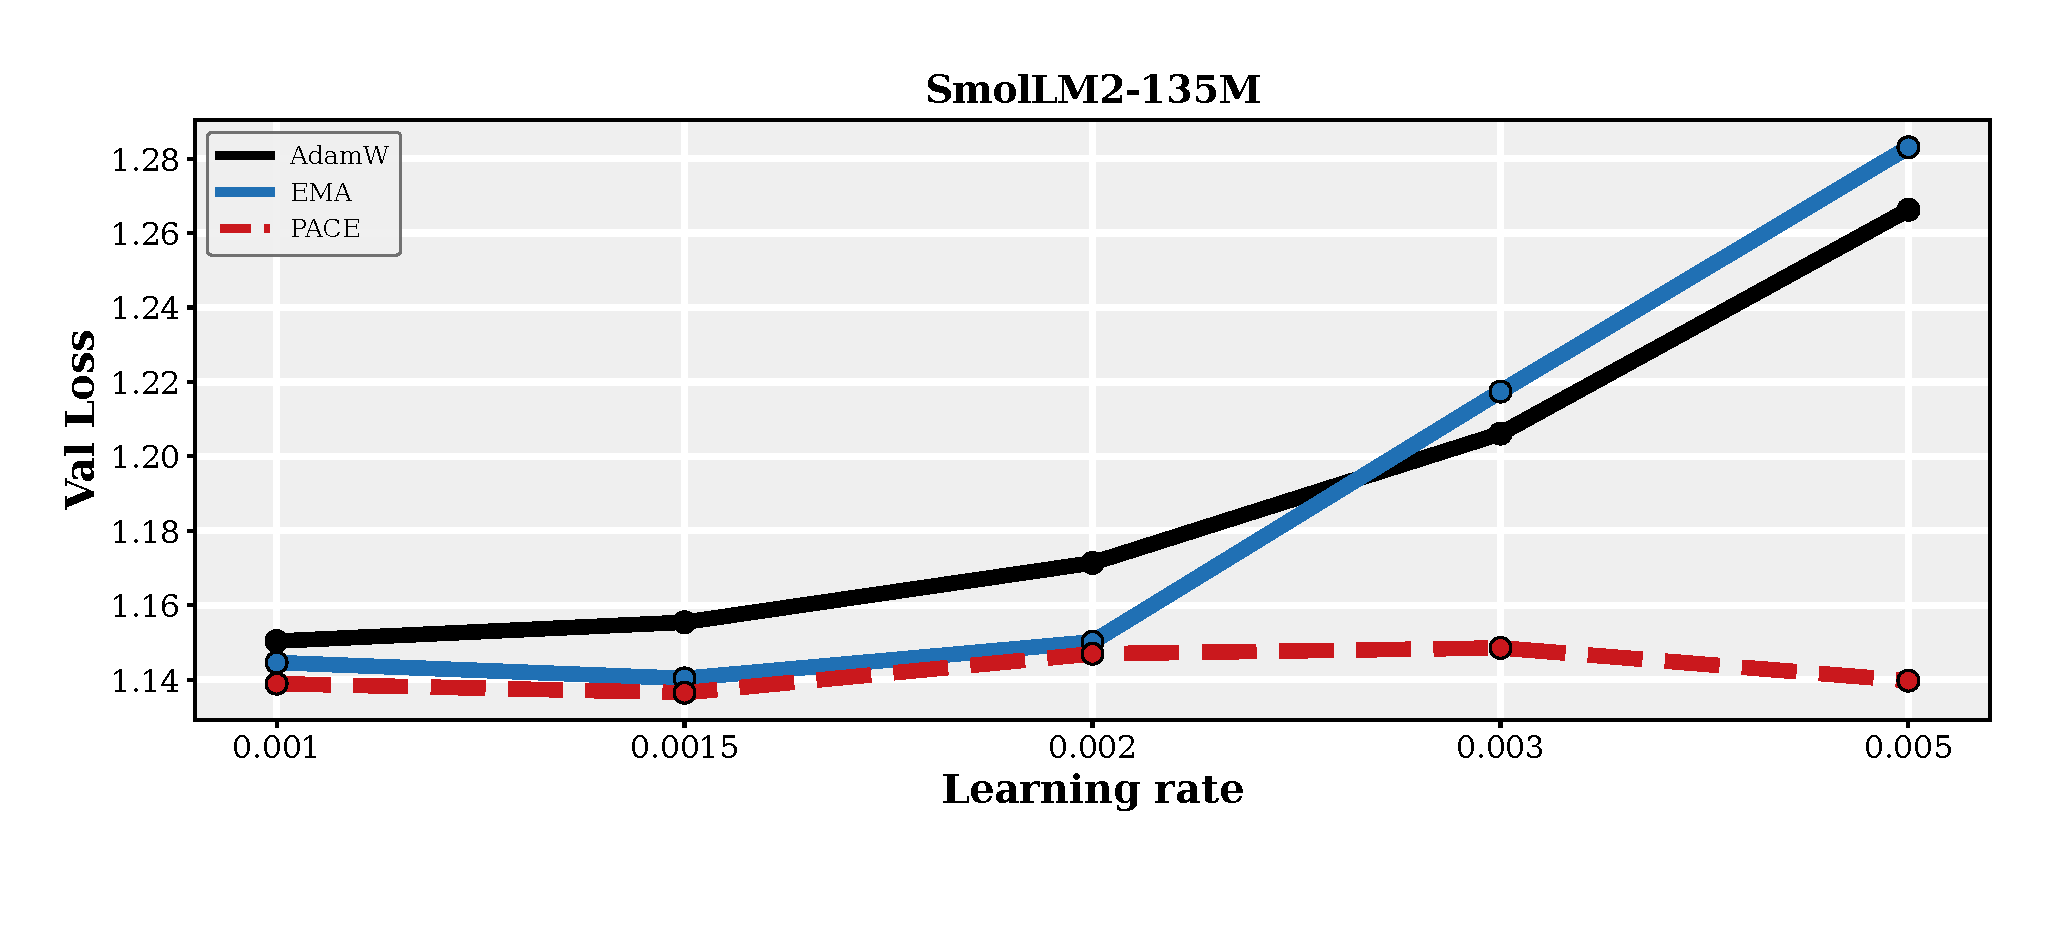
\includegraphics[width=0.676\textwidth]{figures/fig_appendix_wsd_finetune.pdf}
  \caption{\textbf{Fine-tuning across learning rates.} Best validation cross-entropy on SmolLM2-135M for AdamW, EMA, and \pace, with the baselines given their best decay schedule and \pace\ held at a constant learning rate. \pace\ attains the lowest loss at every learning rate, by a margin that widens as the learning rate increases and the baselines degrade.}
  \label{fig:appendix_wsd_finetune}
\end{figure}

\begin{figure}[ht]
  \centering
  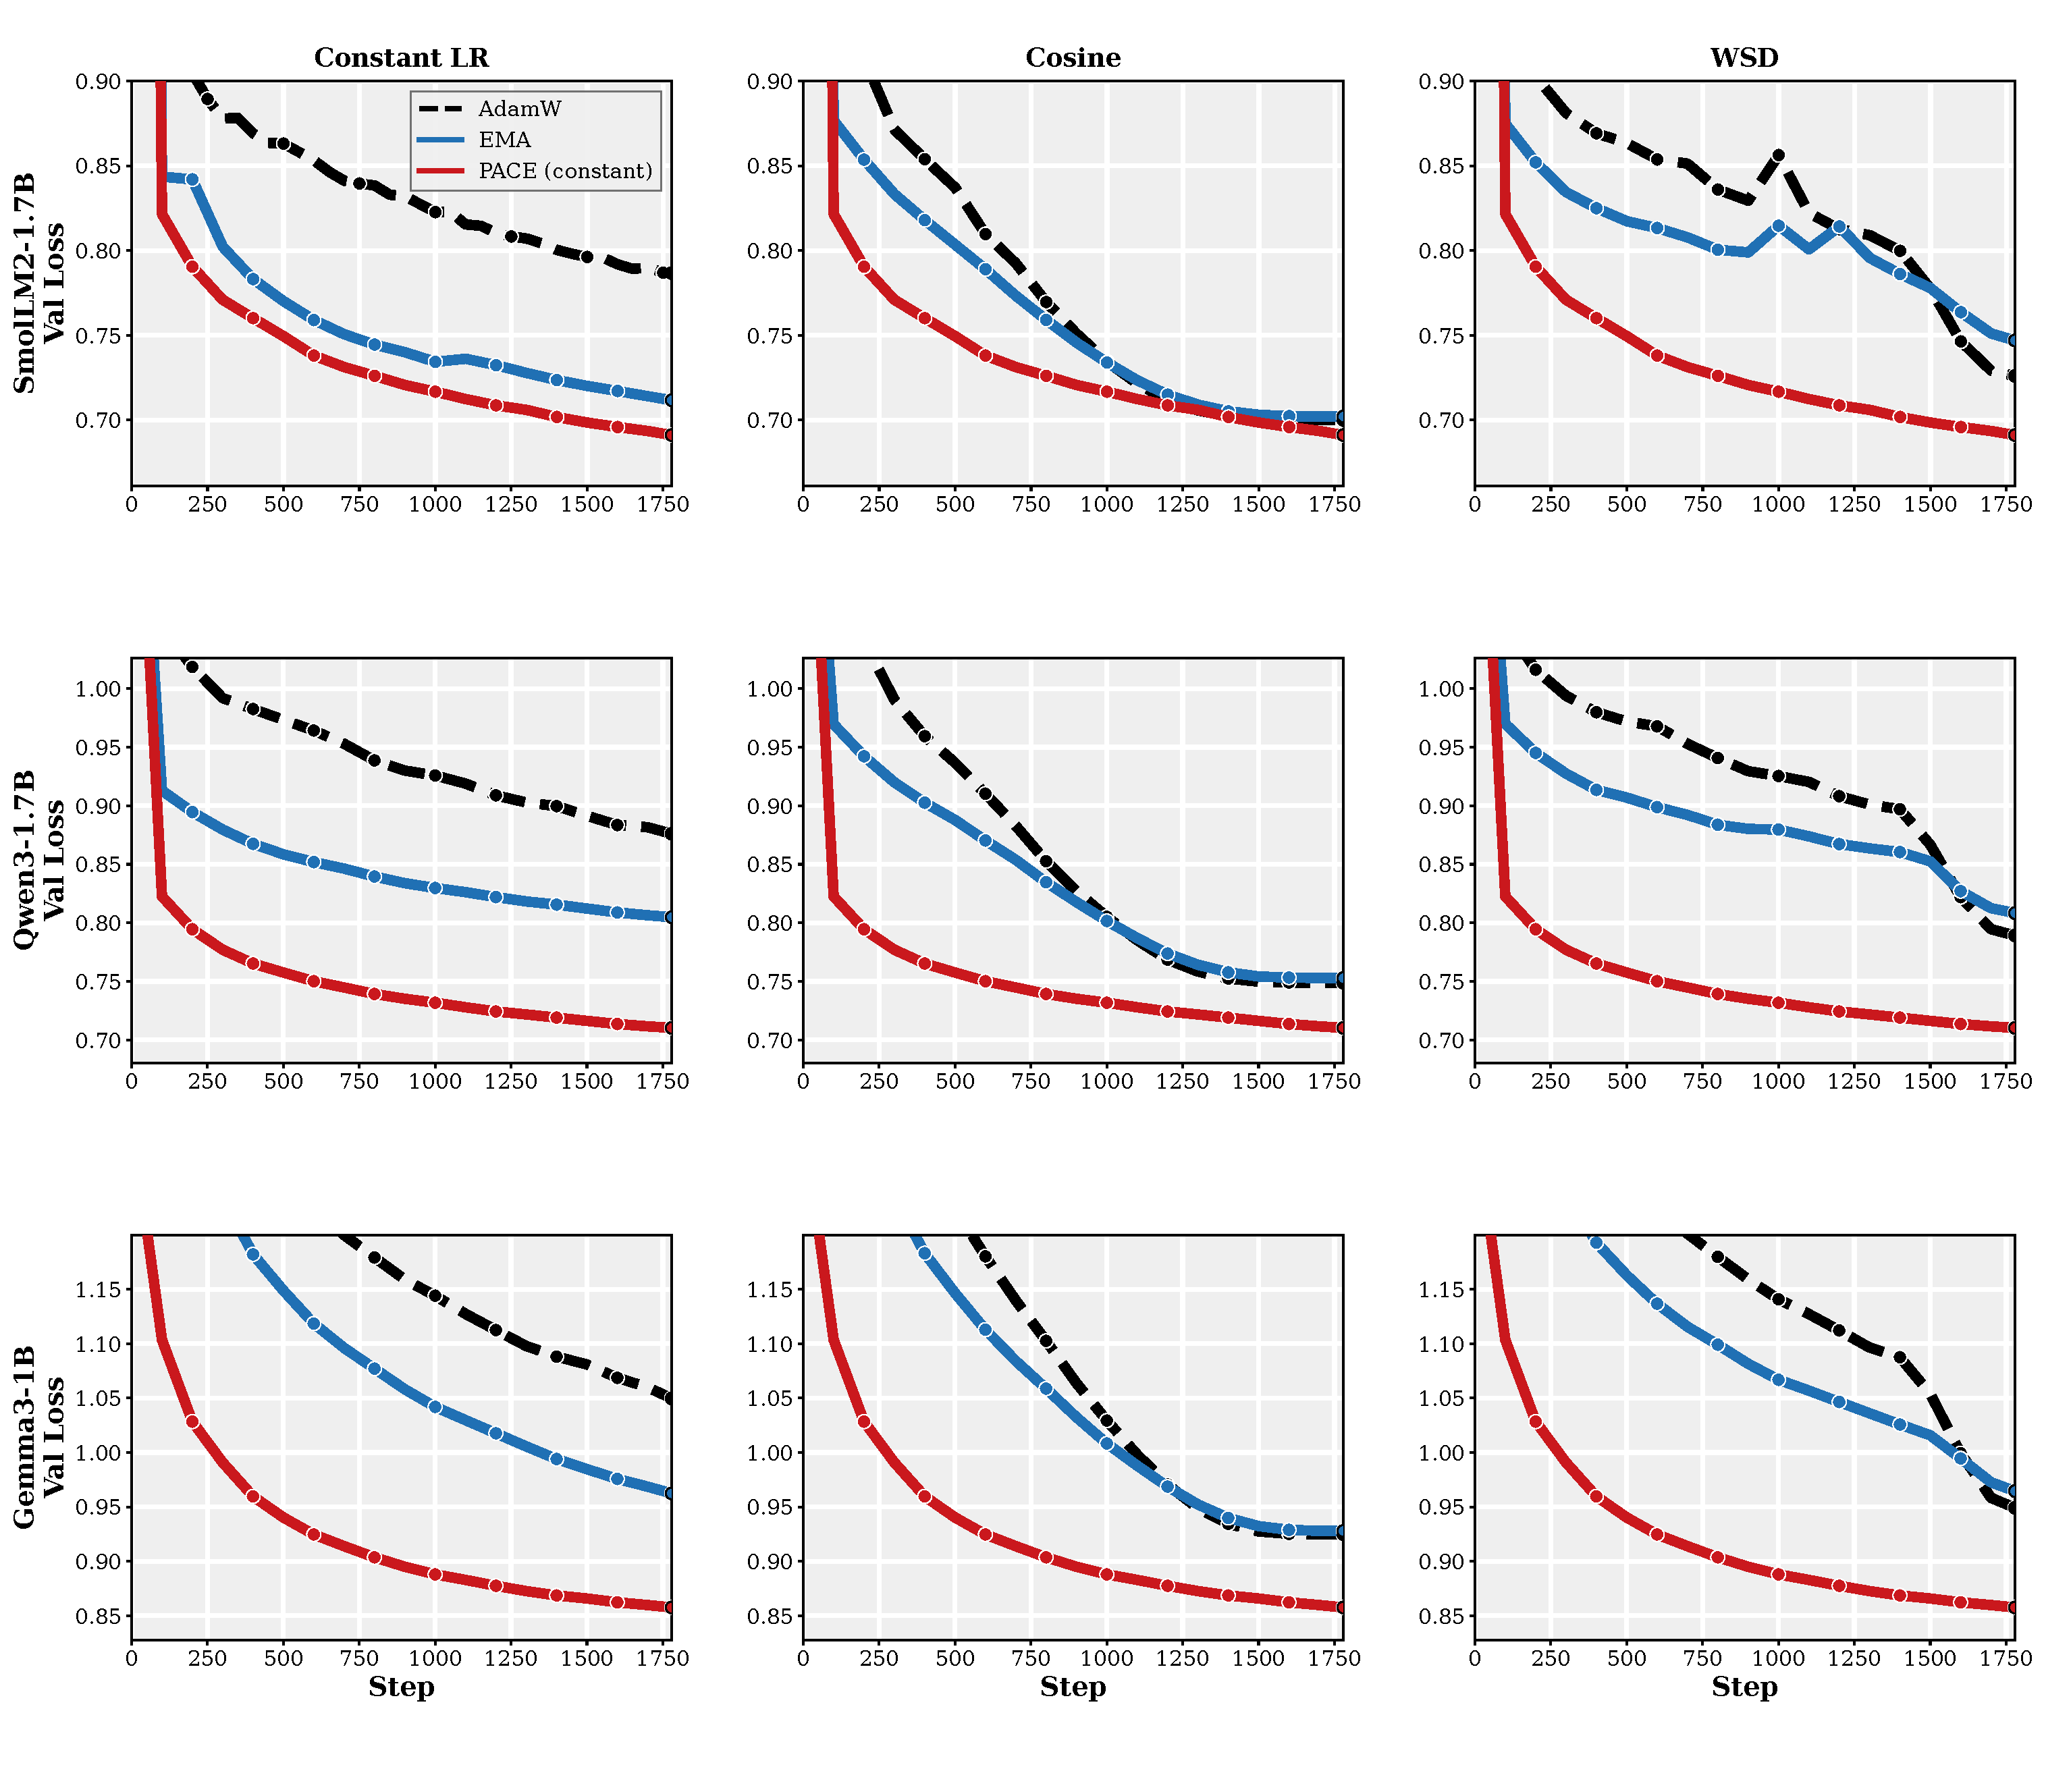
\includegraphics[width=\textwidth]{figures/fig_appendix_fig1_all_schedules.pdf}
  \caption{\textbf{\pace\ against the baselines under every learning-rate
  schedule.} Validation cross-entropy on \texttt{smol-smoltalk}; rows are
  models, columns are the baselines' learning-rate schedule (constant, cosine,
  WSD), with the \pace\ constant-learning-rate run as the reference in each
  panel. \pace\ improves on both baselines under every schedule on all three
  models.}
  \label{fig:appendix_fig1_all_schedules}
\end{figure}

\paragraph{Multi-seed robustness.} Across three seeds, the entire \pace\ band
stays below those of AdamW and \ema\ at every step---under both a constant
learning rate and WSD, on all three models---so the improvement exceeds the
seed-to-seed spread (\Cref{fig:appendix_multiseed_robust}).

\begin{figure}[t]
  \centering
  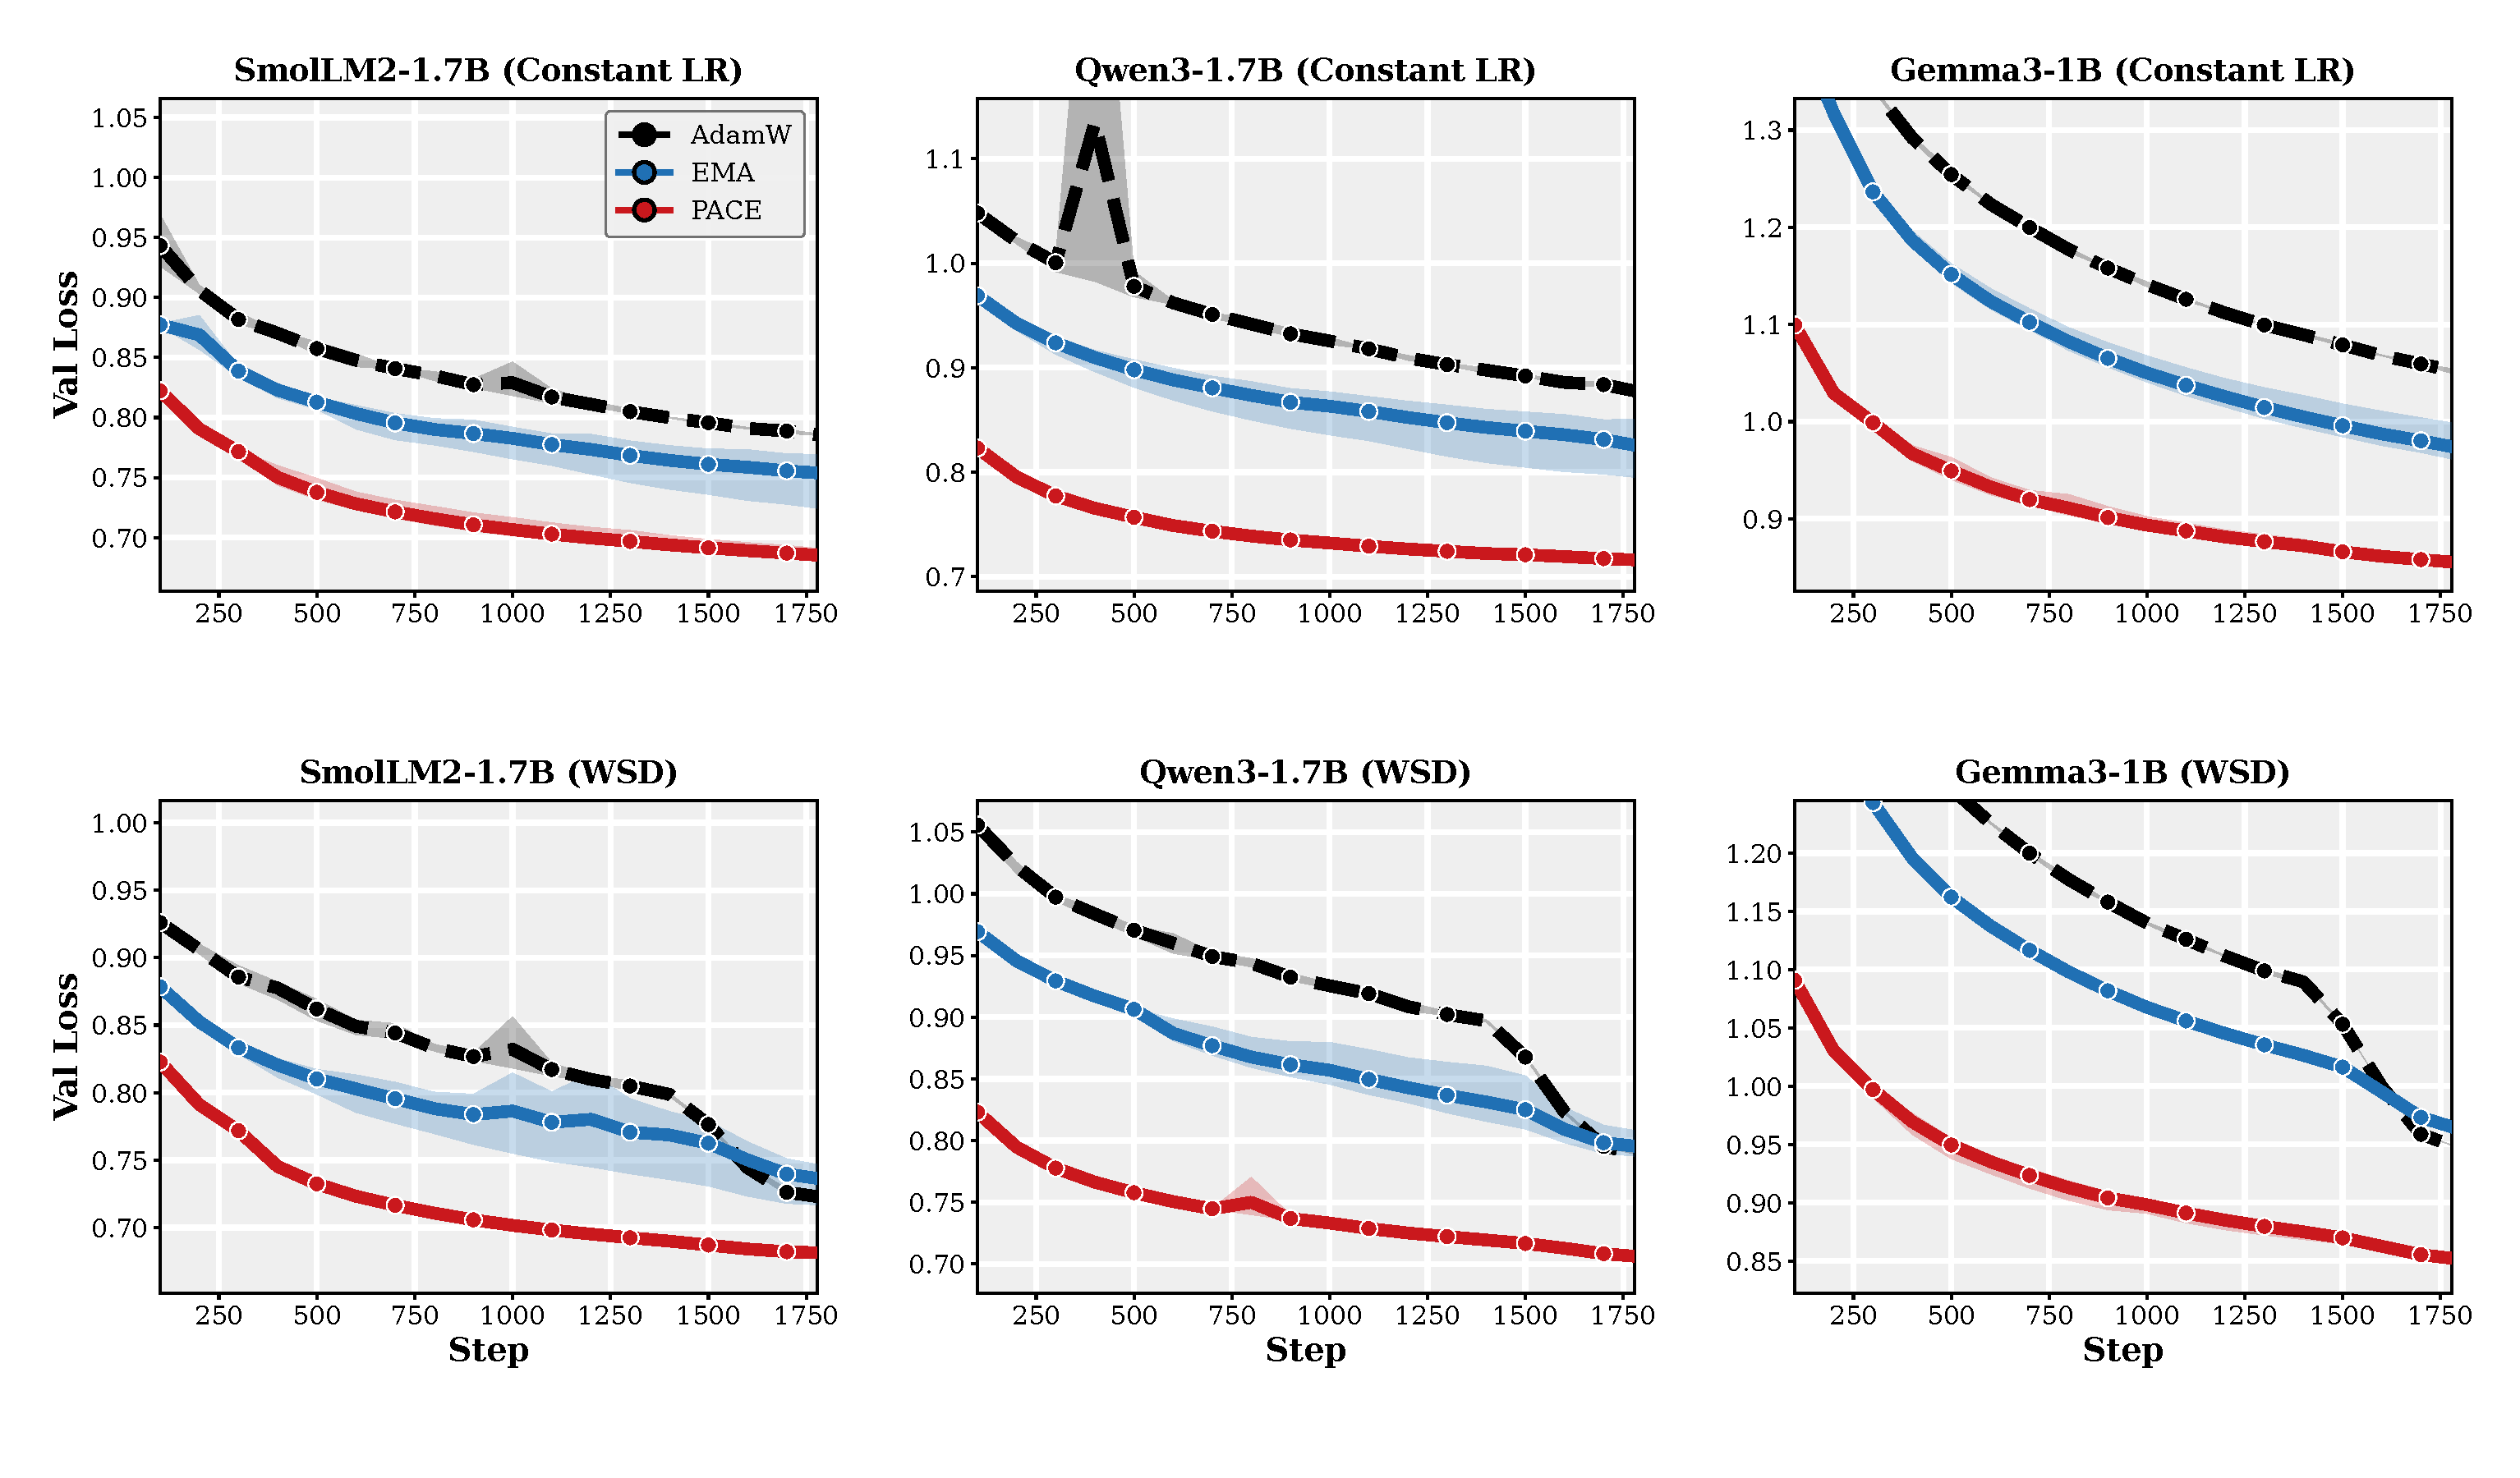
\includegraphics[width=\textwidth]{figures/fig_appendix_multiseed_robust.pdf}
  \caption{\textbf{Multi-seed robustness of fine-tuning.} Across three seeds,
  \pace\ stays below both AdamW and \ema\ on all three models, under both a
  constant learning rate and WSD, by more than the seed-to-seed variation at
  every step.}
  \label{fig:appendix_multiseed_robust}
\end{figure}
